\documentclass[aspectratio=169]{beamer}

\usepackage{beamerthemesplit}
\usepackage{amsmath}
\usepackage{amsfonts}
\usepackage{amssymb}
\usepackage{cancel}
\usepackage{bussproofs}
%% \usepackage{tkz-graph}

\makeatletter
\newcommand{\reallytiny}{\@setfontsize{\srcsize}{2pt}{2pt}}
\makeatother

\mode<presentation>
{
  \usetheme{AnnArbor}
  \usecolortheme{crane}
}

\usepackage[english]{babel}
\usepackage[latin1]{inputenc}
\usepackage{times}
\usepackage[T1]{fontenc}

\title{Combining learning and reasoning for Bio-AI}

\author{Nil Geisweiller}

\institute[SingularityNET OpenCog Foundations]
{
  \begin{center}
    SingularityNET \& OpenCog Foundations\\
    
\includegraphics[scale=0.32]{images/snet_oc.png}
  \end{center}
}
          
\date[OpenCogCon-20]

\begin{document}

\section{Probabilistic Logic Networks for Bio-AI}

\begin{frame}

  %% I have a small presentation, just to warm us up for an actual
  %% discussion.
  
  \maketitle
\end{frame}

\subsection{Why?}

\begin{frame}
  \frametitle{Why?}

  %% If I ask you what would happen if a bird retracts its wings while
  %% flying in the air, you would immediately answer: it's gonna
  %% fall. But have you ever seen a bird retracting its wings while being
  %% the air. Never. So you see you have an incredibly unbalanced data
  %% here, yet you're able to make an extremely good prediction regarding
  %% an outcome that you've never observed.

  %% And the reason is that you're able to utilize background
  %% knowledge that you have that is relevant to the question, here
  %% the background knowledge is about gravity, which we have an
  %% insane confidence about, and in general beneath the background
  %% knowledge, we can have millions/billions of observations to back
  %% that up.
  
  \center{Why combining machine learning and reasoning?}\\[0.5cm]

  \begin{columns}
    \column{5cm}
    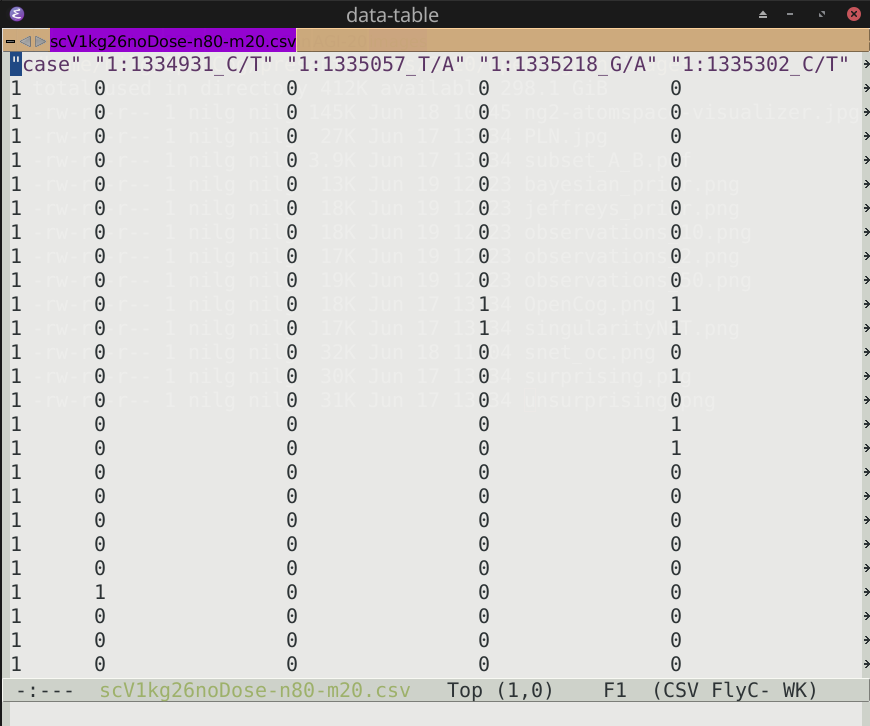
\includegraphics[scale=0.15]{images/table.png}
    \column{0.3cm}
    $\bigotimes$
    \column{5cm}
    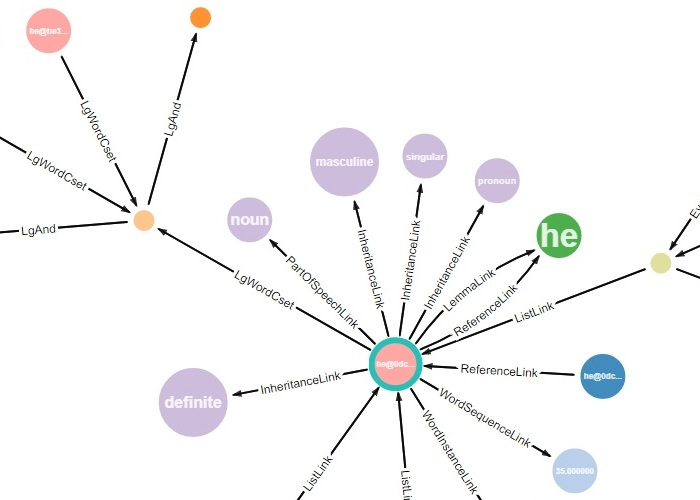
\includegraphics[scale=0.3]{images/atomspace.jpg}
  \end{columns}
  %% \pause
  \center{%% Background knowledge\\
    %% $\Downarrow$\\
    \alert{Massive amount of indirect evidence}\\[0.2cm]
    %% \pause
    \textcolor{red}{Ultimate answer to overfitting}
  }
\end{frame}

\begin{frame}
  \frametitle{Why?}

  %% OK, so in this example I'm using the laws of physics as example
  %% of background knowledge, so what about simulation?

  %% And the problem with simulation is that unless it is fairly
  %% constrained or at the precisely the right scale, etc, it's
  %% basically intractable. Simulation in general can only be done if
  %% we short-cut the calculations, using abstractions. An example of
  %% that would be statistical physics, and its works nice, at this
  %% level. But when we want to go to the levels up, biology, etc,
  %% then it no longer works, and what we actually need are mechanisms
  %% that can creates these abstractions.  And for that we need
  %% reasoning (and learning as well, which is in fact a specialized
  %% form of reasoning).

  %% So what is an abstraction: It is a transformation with a loss of
  %% information that happens to be useful. When you think of the
  %% state of a lamp of instance, you don't need to think about of the
  %% millions of ways photons can come out of this lamp and hit your
  %% retina, you just think of 2 states, is it on or off. And of
  %% course you lose of lot of information, but in our case it is a
  %% good thing because now we only have 1 bit of information to
  %% manipulate.

  \center{What about simulation?}\\[1cm]

  \center{\alert{Impractical without abstractions}\\[1cm]
    %% $\Downarrow$\\[0.5cm]
    \textcolor{red}{Reasoning\\$\Downarrow$\\Abstractions}
  }

\end{frame}

\begin{frame}
  \frametitle{Why?}

  %% And another reason we want to combine reasoning and machine
  %% learning is for meta-learning in general, such as for instance
  %% speeding up learning, but that's a long topic for another time.

  \center{\alert{Help learning (and reasoning)}}\\[1cm]
  
  \begin{itemize}
  \item \color{red}{Reasoning for meta-learning}
    \begin{itemize}
    \item Filter relevant features
    \item Guide optimization
    \end{itemize}
  \item \color{red}{Learning for meta-reasoning}
    \begin{itemize}
    \item Discover inference control patterns
    \item Create contextual Hebbian links
    \end{itemize}
  \end{itemize}

\end{frame}

\section{Learning \& reasoning over the Bio-AtomSpace}

\begin{frame}
  \frametitle{Learning \& reasoning over the Bio-AtomSpace}

  \begin{itemize}
  \item Learning:\\
    \begin{itemize}
    \item MOSES (program evolution)\\
      $\Rightarrow$ \alert{Predictive models}
    \item Pattern Miner (frequent pattern mining)\\
      $\Rightarrow$ \alert{Discover abstractions}
    \end{itemize}
  \item Reasoning:\\
    \begin{itemize}
    \item Pattern Miner
    \item PLN (Probabilistic Logic Networks)\\
      $\Rightarrow$ \alert{Use existing and discovered background knowledge}
    \end{itemize}
  \end{itemize}
  
\end{frame}

\subsection{Example}

\begin{frame}[fragile]
  \frametitle{Example: Knowledge Base}
  \begin{itemize}
  \item From GO
    {\tiny \begin{semiverbatim}
(InheritanceLink
  (ConceptNode "GO:0000001")
  (ConceptNode "GO:0048308"))
    \end{semiverbatim}}
  \item From BioGRID
    {\tiny \begin{semiverbatim}
(EvaluationLink
  (PredicateNode "interacts_with")
  (SetLink 
    (GeneNode "MYPN")
    (GeneNode "ACTN2")))
    \end{semiverbatim}}
  \item From Reactome
    {\tiny \begin{semiverbatim}
(EvaluationLink
  (PredicateNode "has_location")
  (ListLink
    (GeneNode "SCO2")
    (ConceptNode "mitochondrial matrix")))
    \end{semiverbatim}}
  \item From SMP
    {\tiny \begin{semiverbatim}
(MemberLink 
  (GeneNode "GPD1")
  (ConceptNode "SMP0038938"))
    \end{semiverbatim}}
  \end{itemize}
\end{frame}

\begin{frame}[fragile]
  \frametitle{Example: Preprocess KB}

  \begin{itemize}
  \item
    {\tiny \begin{semiverbatim}
(ConceptNode "GO:0005575" (stv 0.960931 0.960846))
    \end{semiverbatim}}
  \item
    {\tiny \begin{semiverbatim}
(ConceptNode "GO:0036343" (stv 0.000203749 0.960846))
    \end{semiverbatim}}
  \item
    {\tiny \begin{semiverbatim}
(SubsetLink (stv 1 1)
  (ConceptNode "GO:1900454" (stv 0.000305623 0.960846))
  (ConceptNode "GO:1900452" (stv 0.000713121 0.960846)))
    \end{semiverbatim}}
  \item
    {\tiny \begin{semiverbatim}
(SubsetLink (stv 0.428571 0.017199)
  (ConceptNode "GO:1900452" (stv 0.000713121 0.960846))
  (ConceptNode "GO:1900454" (stv 0.000305623 0.960846)))
    \end{semiverbatim}}
  \item
    {\tiny \begin{semiverbatim}
(AttractionLink (stv 0.165899 0.213373)
  (ConceptNode "GO:0003013" (stv 0.0110534 0.960846))
  (ConceptNode "GO:0008015" (stv 0.00183374 0.960846)))
    \end{semiverbatim}}
  \end{itemize}

\end{frame}

\begin{frame}[fragile]
  \frametitle{Example: Pattern Miner}

  \center{Discover abstractions (possibly across databases)}

  \begin{itemize}
  \item GO and SMP
    {\tiny \begin{semiverbatim}
(EvaluationLink (stv 0.9998396 1)
  (PredicateNode "nisurp")
  (ListLink
    (LambdaLink
       (VariableNode "$Gene")
       (PresentLink
          (MemberLink
             (VariableNode "$Gene")
             (ConceptNode "SMP0000113"))
          (MemberLink
             (VariableNode "$Gene")
             (ConceptNode "GO:0019371"))))
    (ConceptNode "db-77891201549-p4S0oCVx7m21Nmll")))
    \end{semiverbatim}}
  \item Convert to probabilistic relationship
    {\tiny \begin{semiverbatim}
(Subset (stv 0.73 0.01)
  (ConceptNode "GO:0019371")
  (ConceptNode "SMP0000113"))      
    \end{semiverbatim}}
  \end{itemize}
\end{frame}

\begin{frame}[fragile]
  \frametitle{Example: Inference}
  {\tiny

    \begin{columns}

      \column{5cm}

      \begin{tabular}{|l|l|}
        \hline
        Acronym & Rule \\
        \hline
        CDE & Concept Direct Evaluation \\
        NDI & Negation Direct Introduction \\
        SDI & Subset Direct Introduction \\
        ISDI & Intensional Similarity Direct Introduction \\
        ADI & Attraction Direct Introduction \\
        MTS & Member To Subset \\
        STM & Subset To Member \\
        ISPD & Intensional Similarity Pattern Deduction \\
        \hline
      \end{tabular}

      \column{6cm}

      \begin{tabular}{|l|l|}
        \hline
        Shorthand & Term \\
        \hline
        \textit{<g>} & (Gene "FCGR2B") \\
        \textit{<h>} & (Gene "ITPR3") \\
        \textit{<GO>} & (Concept "GO:0030889") \\
        \textit{<Aging>} & (Concept "Gene Expression Increase with
        Aging") \\
        \hline
      \end{tabular}
    \end{columns}

    \begin{prooftree}
      \AxiomC{(Member \textit{<g>} \textit{<GO>})}
      \RightLabel{(MTS)}
      \UnaryInfC{(Subset (Set \textit{<g>}) \textit{<GO>})}

      \AxiomC{$\hdots$}
      \RightLabel{(NDI)}
      \UnaryInfC{(Not (Set \textit{<g>}))}

      \AxiomC{(Member $\hdots$}
      \RightLabel{(CDE)}
      \UnaryInfC{\textit{<GO>}}
      \RightLabel{(SDI)}
      \BinaryInfC{(Subset (Not (Set \textit{<g>})) \textit{<GO>})}

      \RightLabel{(ADI)}

      \BinaryInfC{(Attraction (Set \textit{<g>}) \textit{<GO>})}

      \AxiomC{$\hdots$}

      \RightLabel{(ISDI)}

      \BinaryInfC{(IntensionalSimilarity (Set \textit{<g>}) (Set \textit{<h>}))}

      \AxiomC{(Member \textit{<h>} \textit{<Aging>})}
      \RightLabel{(MTS)}
      \UnaryInfC{(Subset (Set \textit{<h>}) \textit{<Aging>})}
      
      \RightLabel{(ISPD)}

      \BinaryInfC{(Subset (Set \textit{<g>}) \textit{<Aging>})}

      \RightLabel{(STM)}
      
      \UnaryInfC{(Member (stv 0.13 0.06) \textit{<g>} \textit{<Aging>})}

      %% \UnaryInfC{(Concept "GO:0030889" (stv 0.0008 0.96))}

      %% \AxiomC{(Member \textit{<h>} (Concept "GO:0030889")) $\hdots$}
      %% \RightLabel{(CDE)}
      %% \UnaryInfC{(Concept "GO:0050794" (stv 0.55 0.96))}

      %% \AxiomC{(Subset $A$ $X$) $\hdots$}
      %% \RightLabel{(ADI)}
      %% \UnaryInfC{(Attraction $A$ $B$)}

      %% \AxiomC{$\hdots$}
      
      %% \RightLabel{(ISDI)}

      %% \QuaternaryInfC{(IntensionalSimilarity (stv 0.09 0.67) (Concept
      %%   "GO:0030889") (Concept "GO:0050794"))}

      %% \RightLabel{(ISDI)}
      
      %% \UnaryInfC{(IntensionalSimilarity (stv 0.13 0.14) (GeneNode "FCGR2B") (GeneNode "ITPR3"))}
    \end{prooftree}
  }
  %% 2. concept-direct-evaluation
  %% (ConceptNode "GO:0050794" (stv 0.55316436 0.96080161))
  %% 3. intensional-similarity-direct-introduction
  %% (IntensionalSimilarityLink (stv 0.092158662 0.67346939)(ConceptNode "GO:0030889" (stv 0.00081595186 0.96080161))(ConceptNode "GO:0050794" (stv 0.55316436 0.96080161)))
  %% 4. intensional-similarity-to-member
  %% (IntensionalSimilarityLink (stv 0.13080897 0.13469388)(GeneNode
  %% "FCGR2B")(GeneNode "ITPR3"))
  %% 5. intensional-similarity-property-deduction
  %% (MemberLink (stv 0.12426852 0.061859411)
  %%   (GeneNode "ITPR3")
  %%   (ConceptNode "HAGR increased expression-with-aging GeneSet"))
\end{frame}

\subsection{Status and remaining work}

\begin{frame}
  \frametitle{Status}

  \begin{itemize}
  \item Moderately complex models with MOSES
  \item Simple patterns with Pattern Miner
    \begin{itemize}
    \item Pattern size: 2 conjuncts
    \item GO + SMP dataset: 1M atoms
    \item Time: couple hours
    \end{itemize}
  \item Short inference trees with PLN
    \begin{itemize}
    \item Inference tree size: dozen steps
    \item GO dataset: 650K atoms
    \item Time: couple hours
    \end{itemize}
  \item Focused on longevity
  \end{itemize}
\end{frame}

\begin{frame}
  \frametitle{Difficulties}

  \begin{itemize}
  \item Porting data into the atomspace (consistency checking)
  \item Very resource hungry (millions of atoms)\\
    \begin{itemize}
    \item CPU: 1 single step can take 20+ minutes
    \item RAM: 1 single step can take 64GB+
    \item Need ECAN!
    \end{itemize}
  \item Advanced forms of reasoning\\
    \begin{itemize}
    \item Push PLN to its limits and beyond
    \end{itemize}
  \end{itemize}
\end{frame}

\begin{frame}
  \frametitle{To do}

  \begin{itemize}
  \item Bio-AtomSpace
    \begin{itemize}
    \item Keep importing more data
    \item Experiment with more domains, COVID-19, Cancer, Regenerative Therapy
    \end{itemize}
  \item OpenCog
    \begin{itemize}
    \item Rule-engine
      \begin{itemize}
      \item Multi-threaded Rule Engine
      \item Back-propagate strength (only confidence so far)
      \end{itemize}
    \item PLN
      \begin{itemize}
      \item Fix, add rules
      \item Improve uncertainty calculations
      \end{itemize}
    \item Integrate ECAN
    \item Integrate spatio-temporal reasoning
    \item Experiment with inference control meta-learning
    \end{itemize}
  \end{itemize}
\end{frame}

\end{document}
